\subsection{Music recommendation}
Collaborative filtering is the part of recommender systems that predicts users' preferences for particular items. The major challenge of these methods in predicting users'listening count is that the available user-artist count are usually too few and their performance relies on a good initial estimation of the unknown ratings. This is why we implemented ALS which uses only the known listetning counts and avoids dependencay on initial estimations.
\subsection{Data description}
The training data consists in a matrix $Ytrain$ of size 1774x15082, corresponding to 1774 users and 15802 artists. Element $Ytrain(i,j)$ expresses how many times user i has listened to the artist j. If the value is 0, it means we do not have information for that (user, artist, count) triple.

We are also given the friendship graph of the 1774 users storead as an adjacency matrix.

\subsection{Exploratory Data Analysis}

The listening counts matrix is very sparse with a density of only $0.0026\%$, correspinding to 
69617 entries.
The highest count is 352698, the average listening count per user is  5.52 and the average listening count per artist is 5.46.

A histogram of counts, shown in Fig\ref{fig:count_distribution} tells us that the listening counts follow a heavy tail distribution.
The long tail contains a small number of popular items, the well-known
artists, and the rest are located in the heavy tail.
One method to transform skewed data such that it becomes more gaussian distributed is to use the Box-Cox transform. In our case, we can choose $lamda=0$ since for us  y values are very high and > 0. This transformation will make the distances between listening counts much smaller and will reduce the influence on RMSE of the (user,artist,count) triples in the long tail. 

\begin{figure}[h]
  \centering
  \begin{subfigure}[b]{0.45\textwidth}
   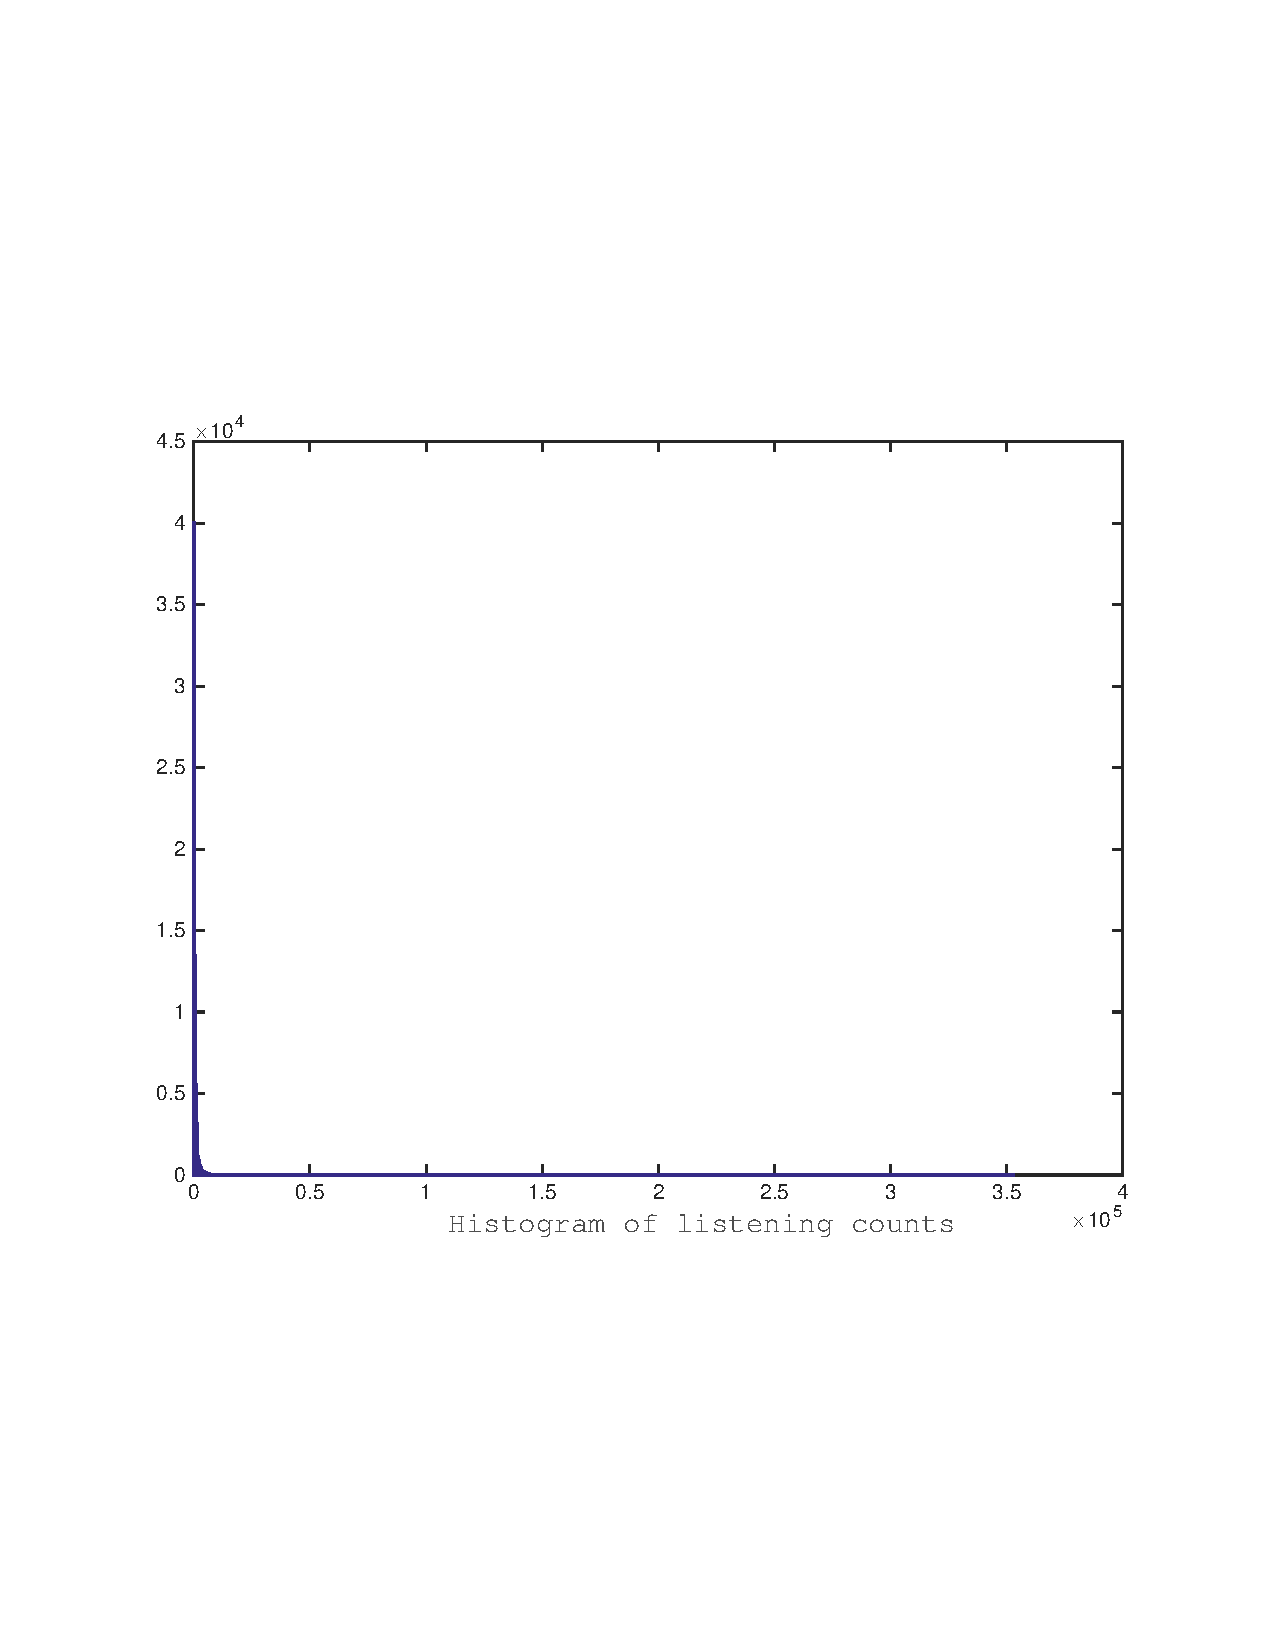
\includegraphics[width=\textwidth]{figures/histYtrain_crop.pdf}
    \caption{Before data transformation}
  \end{subfigure}
  \begin{subfigure}[b]{0.45\textwidth}
    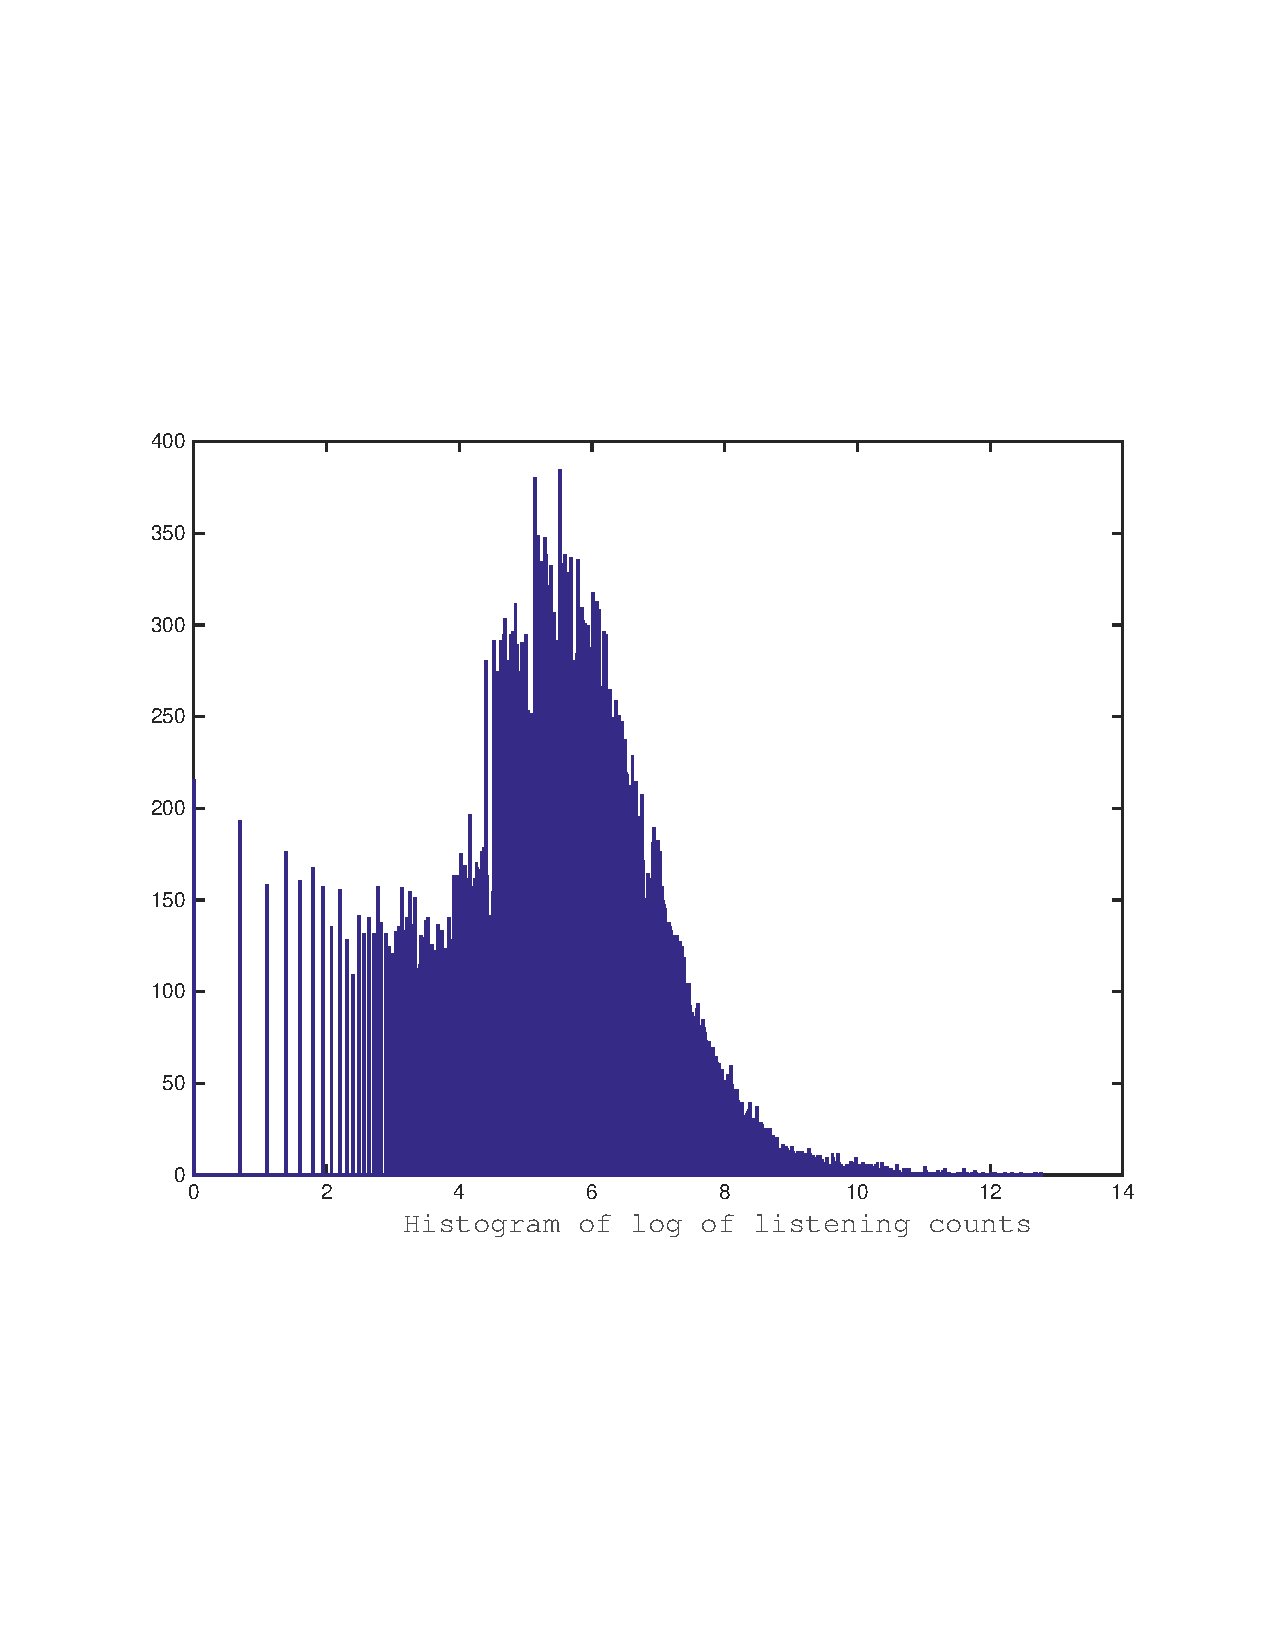
\includegraphics[width=\textwidth]{figures/histLogYtrain_crop.pdf}
    \caption{Negative image.}
  \end{subfigure}
  \caption{After data transformation}
  \label{fig:count_distribution}
\end{figure}

\begin{figure}[h]
  \centering
  \begin{subfigure}[b]{0.45\textwidth}
   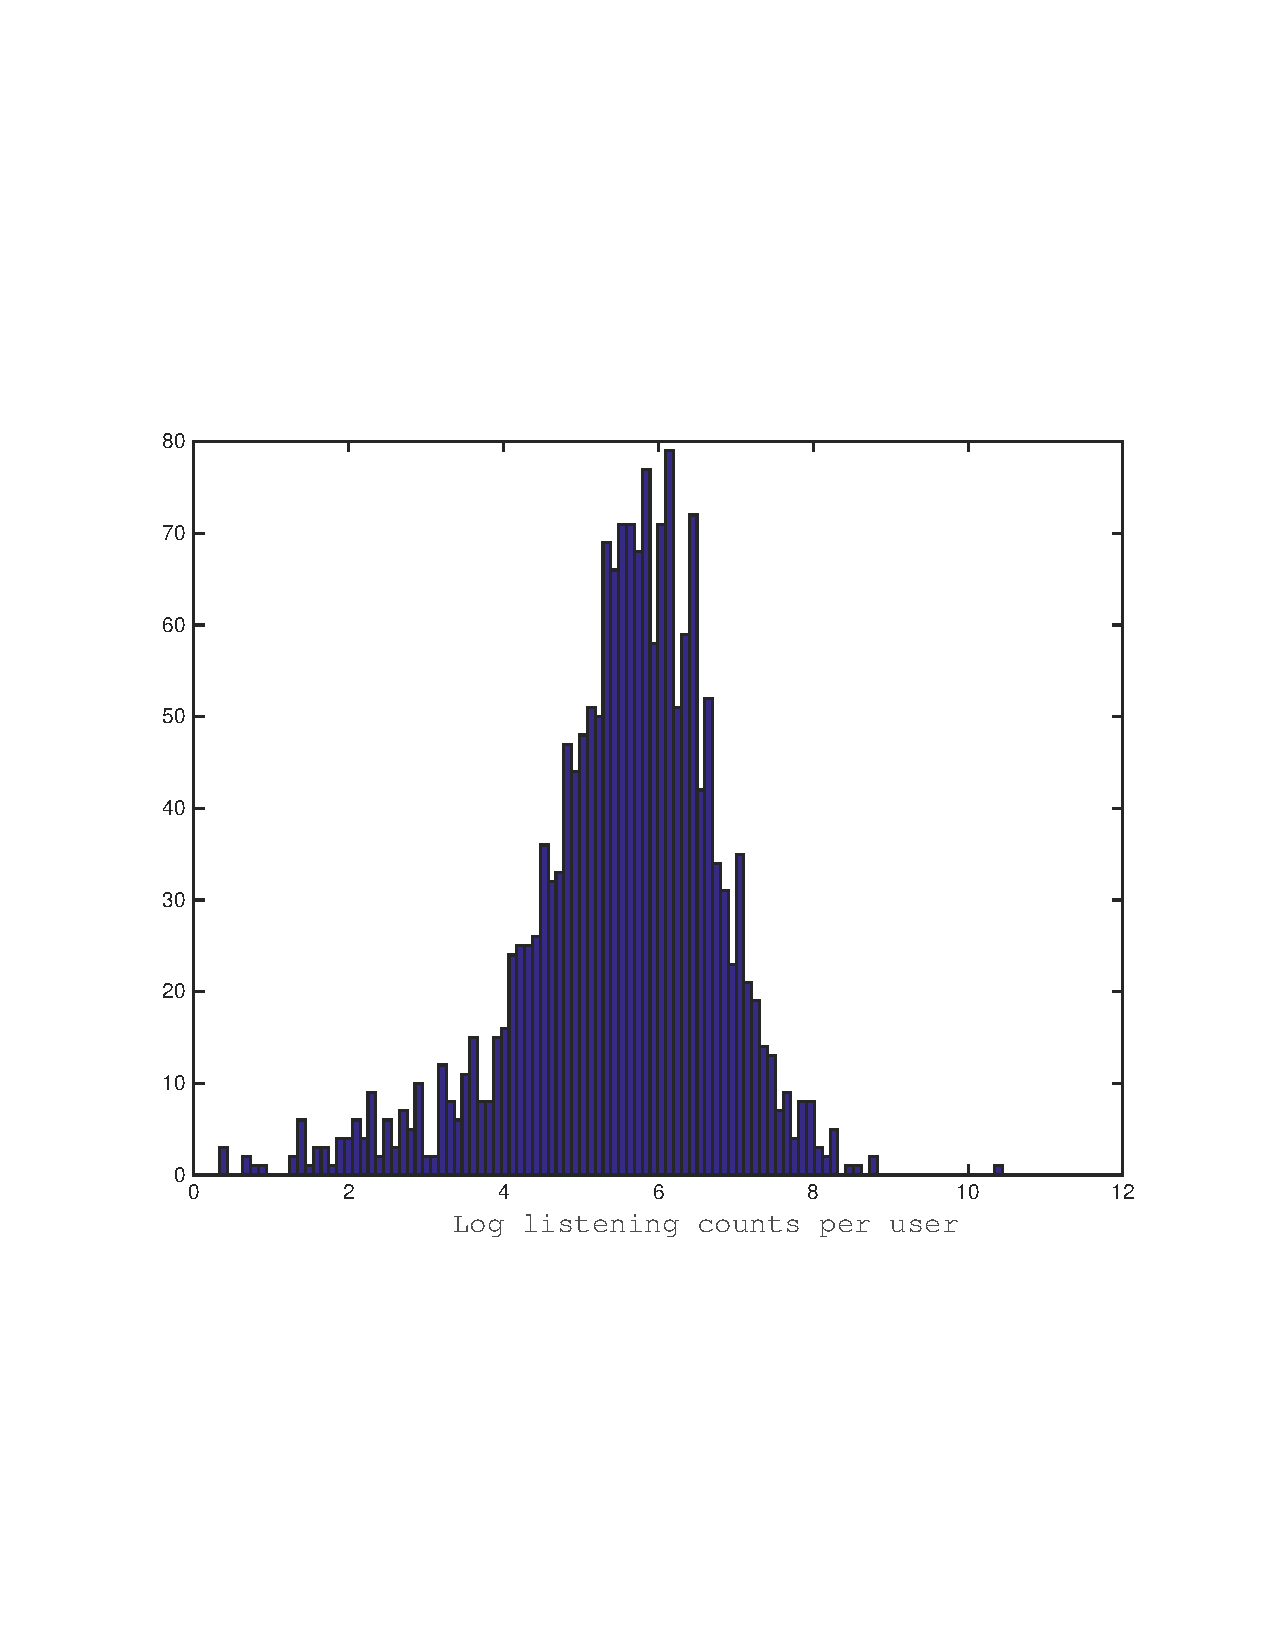
\includegraphics[width=\textwidth]{figures/histCountPerUser.pdf}
    \caption{}
  \end{subfigure}
  \begin{subfigure}[b]{0.45\textwidth}
    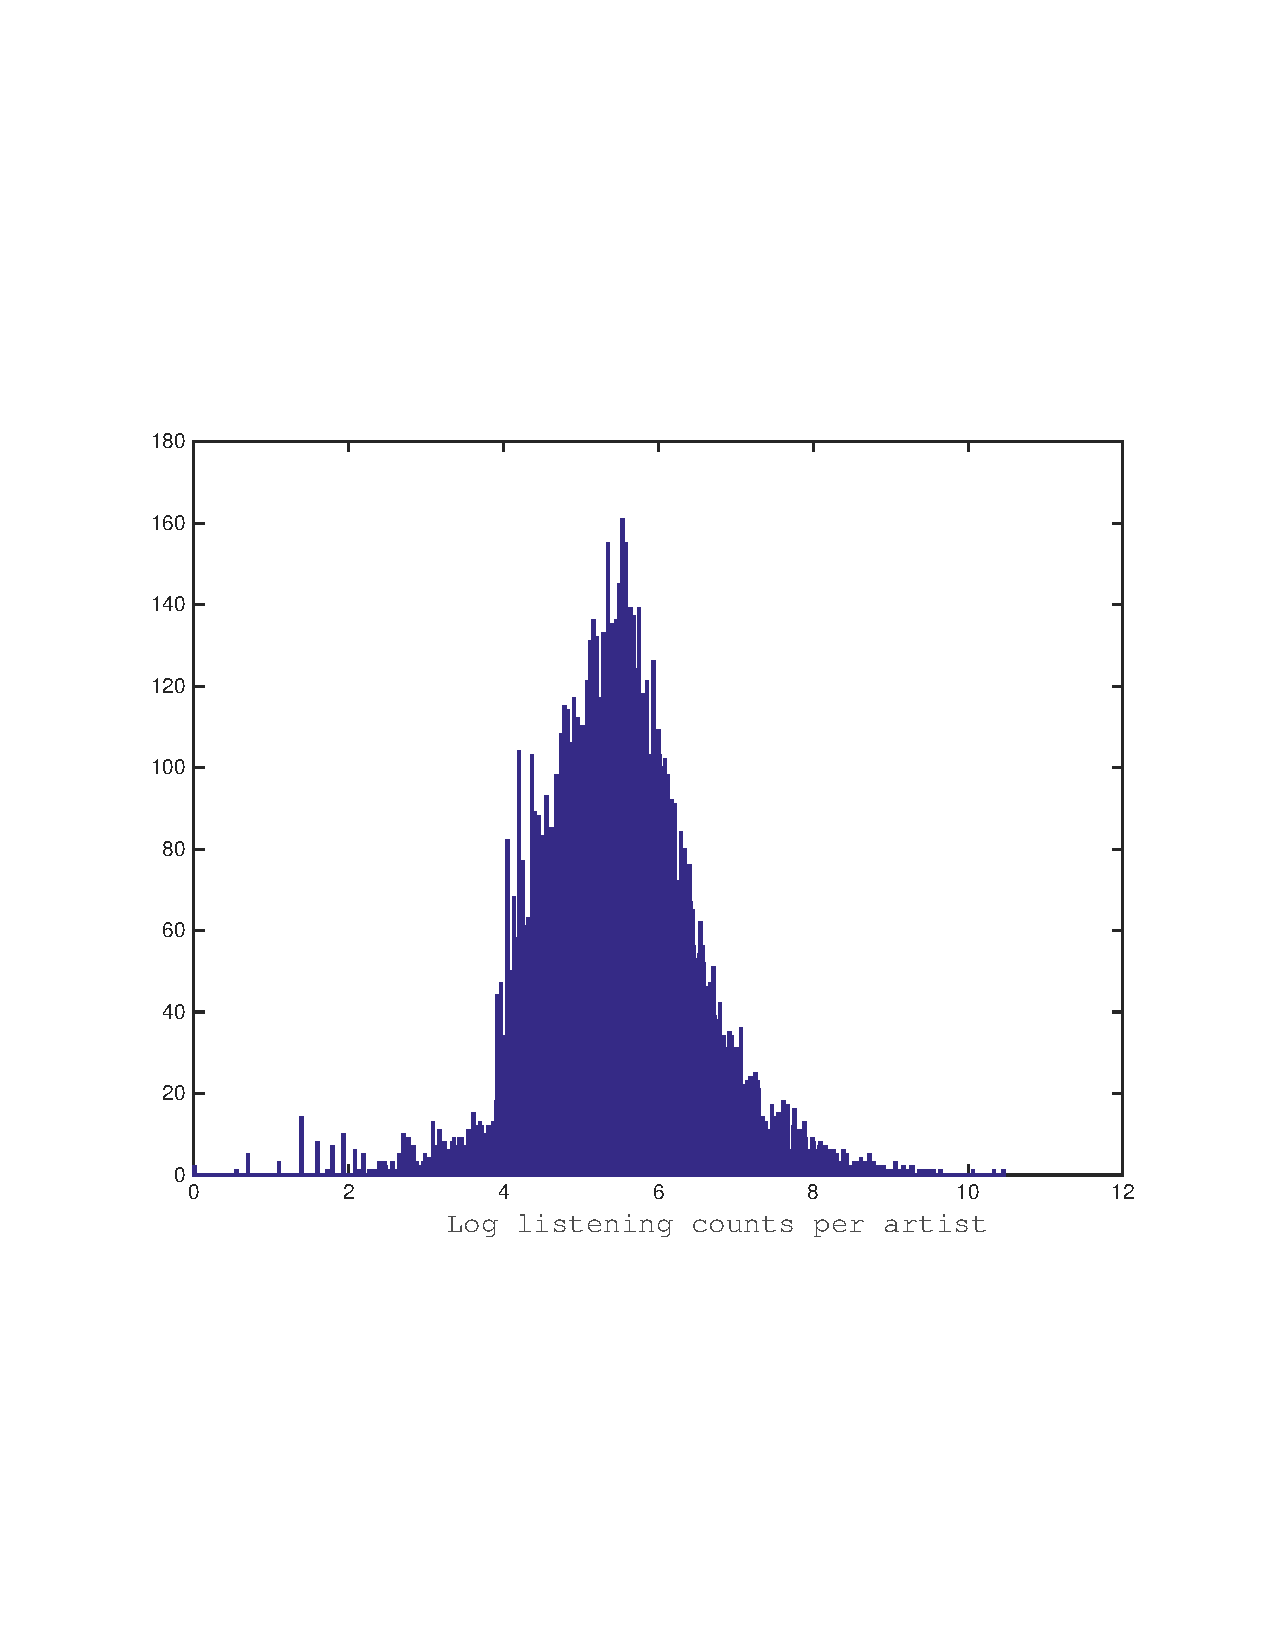
\includegraphics[width=\textwidth]{figures/histCountPerArtist.pdf}
    \caption{}
  \end{subfigure}
  \caption{Per user and per artist log of listenining count distribution}
  \label{fig:user_artist_distribution}
\end{figure}
1262 artists had 0 listening counts.

 
\subsection{Task 1}
20 per cent of the entries in Ytrain were kept for testing and the rest of the entries
were kept for training and validation using 10-fold cross validation.
Splitting the data was  more difficult since we needed to make sure we do not
remove completely the counts of an user or the counts of an artist.
\subsubsection{KNN}
\subsubsection{ALS}

\subsubsection{logALS}
\subsubsection{Kmeans}

\subsection{Task 2}
\subsubsection{Friendship information}
Regarding the friendshiop information, we noticed there are 22 connected components, but many of them contained.
1776 nodes and 22904 edges.
Using Vincent D Blondel, Jean-Loup Guillaume, Renaud Lambiotte, Etienne Lefebvre, Fast unfolding of communities in large networks, in Journal of Statistical Mechanics: Theory and Experiment 2008 (10), P1000 and the Gephi tool to find properties of the graph, it suggested it has about
32 communities, of which 8 had more than 150 members and the others being very small. (22 connected components, of which 20 are very small < 50 users.) This was run to give us an idea of the number of clusters we could use in Kmeans.


\subsection{Summary}



